%!TEX root = main.tex
\begin{figure*}[ht!]
  \centering
  \vspace{-5pt}
  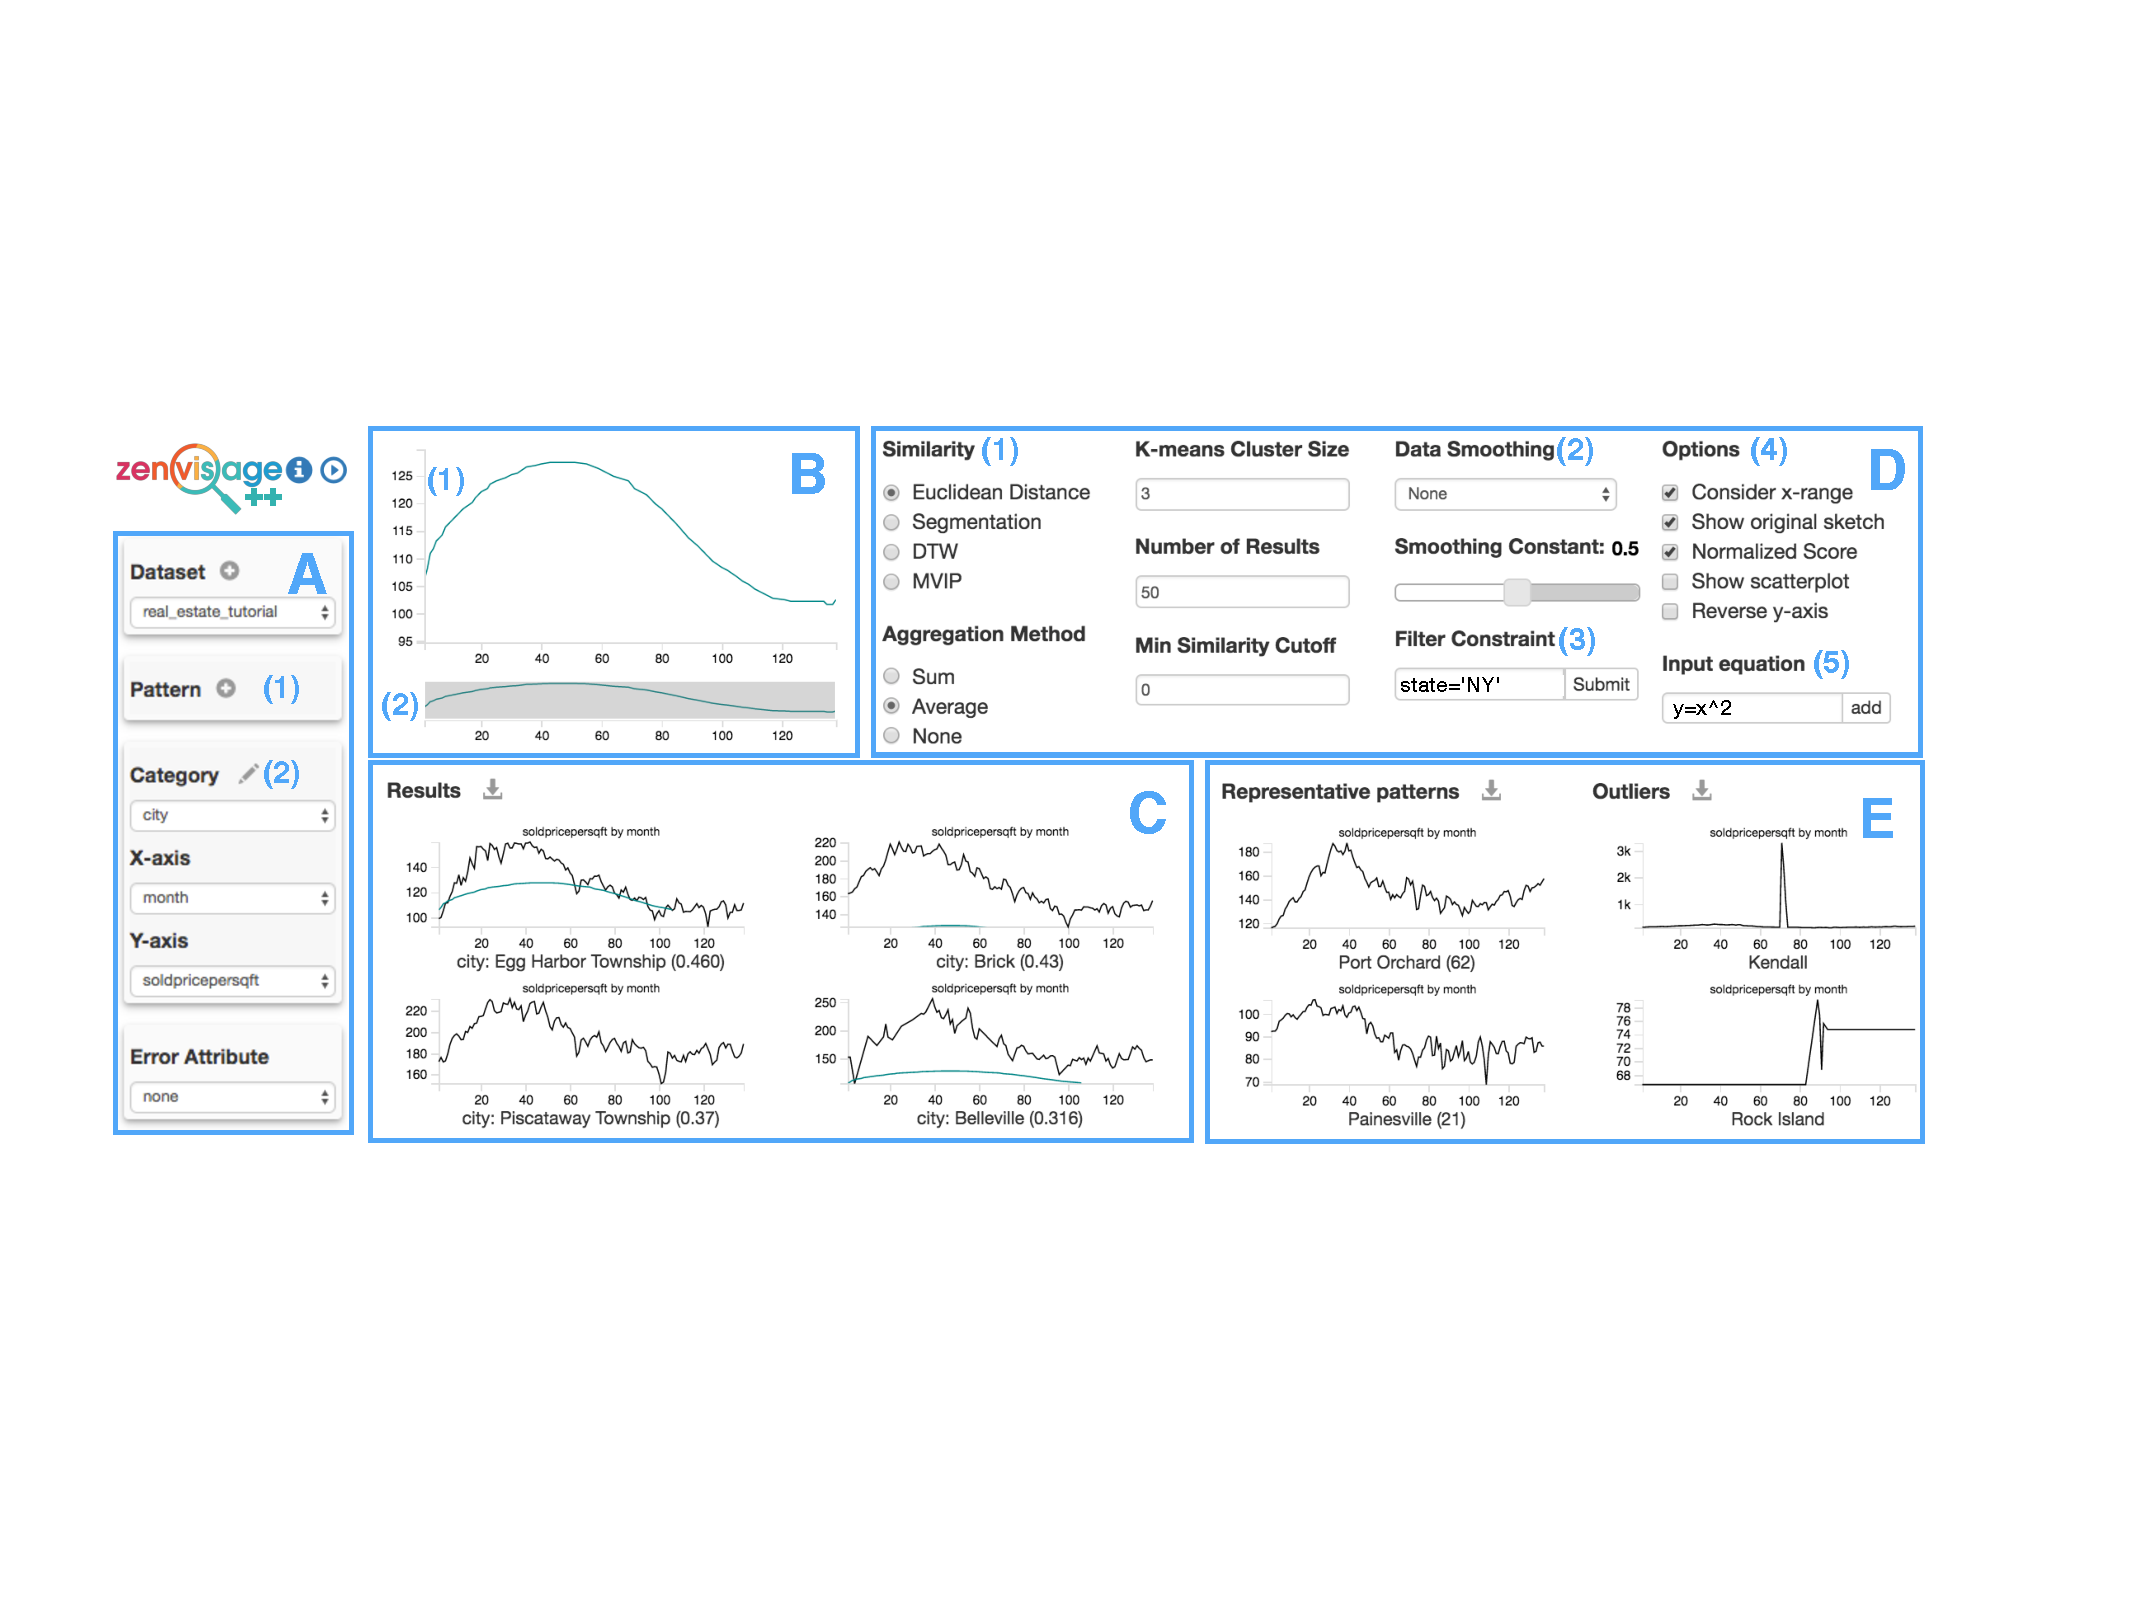
\includegraphics[width=0.95\linewidth]{figures/zvpp_system.pdf} %5.5
  \vspace{-5pt}\caption{\change{The \zvpp system consist of : (A) data selection panel (where users can select visualized dataset and attributes), (B) query canvas (where the queried data pattern is submitted and displayed), (C) results panel (where the visualizations most similar to the queried pattern is displayed as a ranked list), (D) control panel (where users can adjust various system-level settings), and (E) recommendation (where the typical and outlying trends in the dataset is displayed).}}
  \label{zvOverview}
  \vspace{-5pt}
\end{figure*}
\section{System-level Participatory Design Findings\label{sec:pd_findings}}
%All of the three domains described in the previous section recognized the need for a VQS. As discussed in Section~\ref{sec:methods},
%we worked closely with participants to develop features to address their problems and challenges.
\change{
  Holzblatt and Jones~\cite{HoltzblattJones} describes contextual inquiry as a technique that forms the basis for ``\textit{developing a system model that will support user's work}'' that subsequently ``\textit{fosters participatory design}''. Given the need for a VQS highlighted in contextual inquiry interviews, we further distill a list of VQS features by working closely with participants to develop features to address their problems and challenges. In this section, we first reflect on our participatory design (PD) methodology
  to introduce the PD findings, then we provide a high-level system overview of our PD product, \zvpp.

  \subsection{The Collaborative Feature Discovery Process}
  \par Throughout the PD process, we identified various subtasks based on the scientist's workflow and elicited intermediate feedback.
  Bodker et. al.~\cite{BodkerGronbaek} cites the importance of encouraging user participation and creativity in cooperative design through different techniques, such as future workshops, critiques, and situational role-playing. Similarly, our PD objective was to collect as many comprehensive list of feature proposals, inclusive across different domains, leading to the added features listed in Table~\ref{bigfeaturetable}. Given the highly-evolving, unstructured nature of exploratory data analysis (CITE), this technique comes with its advantages and limitations, since users request (or lack thereof) may not always translate to a direct need. For instance, we found that introducing the newly-added features from \zvpp that addressed a particular use case often results in discovering an unexpected practice usage of the feature with other groups of participants. Having feature proposals inspired by multiple use cases can also lead to more generalized design choice. For example, we spoke to astronomers who wanted to eliminate sparse time series from their visual queries. In the same week, we spoke to material scientists who expressed a need for inspecting only solvents with properties above a certain threshold. Through these use cases, data filtering arose as a crucial, common operation that we needed to incorporate into \zvpp in order to support these class of queries.
  \par While our collective brainstorming led to the cross-pollination and generalization of features, this technique can also lead to unnecessary features that result in wasted engineering efforts. During the design phase, there were numerous problems and features proposed by participants, but not all were incorporated in the tool. Based on our meeting logs with participants, we found that the reasons for not taking a feature from the design stage to the implementation stage includes:

  \begin{denselist}
  \item Nice-to-haves: One of the most common reasons for unincorporated features comes from participant's requests for nice-to-have features. The amount of nice-to-have features that one could envision for the tool is endless. We use
  two criteria to heuristically judge whether to implement a particular feature:
  \begin{enumerate}[leftmargin=*]
  \item \textit{Necessity:} Without this feature, can the analyst still work with this dataset using our tool and achieve what they want to do?
  \item \textit{Generality:} If this feature was implemented, will it benefit only this specific use case or be potentially useful for other applications as well?
  \end{enumerate}
  \item ``One-shot'' operations: We decided not to include features that were ``one-shot'' operations that only needed to be performed once during the analysis workflow. For example, certain data preprocessing operations such as filtering null values only needed to be performed once unlike the data smoothing feature that we added, which was a preprocessing step that could be iteratively performed along with other operations in the VQS. This design choice is specific to our VQS design study.
  \item Substantial research or engineering effort: Some proposed features do not make sense in the context of VQS. For example, the \matsci group proposed functional fitting to obtain fitting coefficients. Other features requires a completely different set of research questions. For example, the question of how to properly compute similarity between time series with non-uniform number of datapoints arose in the astronomy and genetics use case, but requires the development of a novel distance metric or algorithm that is out of the scope of the RQs of our design study.
  \item Underdeveloped ideas: Other feature requirements came from casual specification that were underspecified. For example, A1 wanted to look for objects that have deficiency in one band and high emission in another band, but what brightness levels qualifies as a deficiency is ambiguous.
  \end{denselist}
  \par Failure to identify these early signs in the design phase may result in feature implementations that turn out not to be useful for the participants. Given exhaustive nature of Table~\ref{bigfeaturetable}, each motivated by example use cases from one or more domains, we organized the features list in terms of the sensemaking framework described in Section~\ref{sec:sensemaking} and evaluated its effectiveness in the evaluation study in Section~\ref{sec:eval_findings}.
}
%Our experimental evaluation shows that some of our feature choices also suffer from these pitfalls. For example, we incorporated the feature to reverse the y-axis so that astronomers could better understand magnitude measurements (as larger magnitudes counter-intuitively corresponds to dimmer objects). In hindsight, the feature was not crucial for the analysis since another derived measure present in dataset could be selected instead and the feature was solely specific to the astronomy use case. In the end, we found that this feature was not used by any of the participants (including the proposer) in the user study.

% These longitudinal collaboration led to a list of features that help support these subtasks. Given the , we encouraged participants to ----how VQS features could assist them in their PD
%  which is later organized into a ------ framework in Section ----, and evaluated in ----

% collective brainstorm exercise
% partnership
% during this ---- `what-if'
% with the participant's dataset
% The result of our ----
% The goal of our participatory design process was to collect brainstorm --- a comphrensive list of ----
% encourage creativity and inclusiveness across domains---
% EDA is inherently unstructured process, highly evolving ,etc
%incrementally incorporated and improved over time as described in the Figure~\ref{timeline} timeline
\change{
  \subsection{System\label{sec:system}}
  The \zvpp interface is organized into 5 major regions that dynamically updates upon user interactions. Typically, analysts begin their analysis by selecting the dataset and attribute to visualize in the \emph{data selection panel} (Figure~\ref{zvOverview}A). Then, they can specify a pattern of interest as a query (hereafter referred to as \emph{pattern query}), through either sketching, inputting an equation, uploading a data pattern, or dragging and dropping an existing visualization, displayed on the \emph{query canvas} (Figure~\ref{zvOverview}B). \zvpp performs shape-matching between the queried pattern and other possible visualizations and returns a ranked list of visualizations that are most similar to the queried pattern, displayed in the \emph{results panel} (Figure~\ref{zvOverview}C). At any point during the analysis, analysts can adjust various system-level settings through the \emph{control panel} (Figure~\ref{zvOverview}D) or browse through the list of \emph{recommendations} provided by \zvpp (Figure~\ref{zvOverview}E). Our \zvpp system is open source and available at: \url{github.com/[Annonymized for Submission]}.
}
\begin{table*}[ht!]
  \begin{tabular}{|l|l|l|l|l|}
\hline
Component & Feature & Purpose & Task Example & \begin{tabular}[c]{@{}l@{}}Similar Features\\ in Past VQSs\end{tabular} \\ \hline
\rowcolor[HTML]{AADFFD}
\cellcolor[HTML]{AADFFD} & \begin{tabular}[c]{@{}l@{}}Query by Sketch\\ (Figure \ref{zvOverview}B1)\end{tabular} & \begin{tabular}[c]{@{}l@{}}Freehand sketching for \\ specifying pattern query.\end{tabular} & \begin{tabular}[c]{@{}l@{}}\A Find patterns with a peak \\ and long-tail decay that\\ may be supernovae candidates.\end{tabular} & \begin{tabular}[c]{@{}l@{}}All include sketch \\ canvas except~\cite{Hochheiser2004}.\end{tabular} \\ \cline{2-5}
\rowcolor[HTML]{AADFFD}
\cellcolor[HTML]{AADFFD} & \begin{tabular}[c]{@{}l@{}}Input Equation\\ (Figure \ref{zvOverview}A1)\end{tabular} & \begin{tabular}[c]{@{}l@{}}Specify a exact functional \\ form as a pattern query \\ (e.g., y=$x^2$).\end{tabular} & \begin{tabular}[c]{@{}l@{}}\M Find patterns exhibiting \\ inversely proportional \\ chemical relationship.\end{tabular} & ---- \\ \cline{2-5}
\rowcolor[HTML]{AADFFD}
\multirow{-3}{*}{\cellcolor[HTML]{AADFFD}\begin{tabular}[c]{@{}l@{}}Pattern\\ Specification\end{tabular}} & \begin{tabular}[c]{@{}l@{}}Pattern Upload\\ (Figure \ref{zvOverview}D2)\end{tabular} & \begin{tabular}[c]{@{}l@{}}Upload a pattern consisting\\ of a sequence of points as \\ a query.\end{tabular} & \begin{tabular}[c]{@{}l@{}}\A Find supernovae based on \\ previously discovered sources.\end{tabular} & \begin{tabular}[c]{@{}l@{}}Upload CSV\\ \cite{mohebbi2011google}\end{tabular} \\ \hline
\rowcolor[HTML]{AADFFD}
\cellcolor[HTML]{AADFFD} & \begin{tabular}[c]{@{}l@{}}Smoothing\\ (Figure \ref{zvOverview}D2)\end{tabular} & \begin{tabular}[c]{@{}l@{}}Interactively adjusting the level \\ of denoising on visualizations,\\ effectively changing the degree\\ of shape approximation when \\ performing pattern matching.\end{tabular} & \begin{tabular}[c]{@{}l@{}}\textbf{A, M:} Eliminate patterns \\ matched to spurious noise.\end{tabular} & \begin{tabular}[c]{@{}l@{}}Smoothing\\ ~\cite{Mannino2018}\\ Angular slope queries\\ ~\cite{Hochheiser2004}\\ Trend querylines\\ ~\cite{ryall2005querylines}\end{tabular} \\ \cline{2-5}
\rowcolor[HTML]{AADFFD}
\cellcolor[HTML]{AADFFD} & \begin{tabular}[c]{@{}l@{}}Range \\ Selection\\ (Figure \ref{zvOverview}B2, D4)\end{tabular} & \begin{tabular}[c]{@{}l@{}}Restrict to query only in \\ specific x/y ranges of interest \\ through brushing selected\\ x-range and filtering \\ selected y-range.\end{tabular} & \begin{tabular}[c]{@{}l@{}}\A Matching only around \\ shape exhibiting a peak.\\ \M Matching only around \\ shape region that exhibit linear\\ or exponential relationships\end{tabular} & \begin{tabular}[c]{@{}l@{}}Text Entry\\ ~\cite{wattenberg2001sketching,Mannino2018}\\ Min/max boundaries\\ ~\cite{ryall2005querylines}\\ Range Brushing\\ ~\cite{Hochheiser2001}\end{tabular} \\ \cline{2-5}
\rowcolor[HTML]{AADFFD}
\multirow{-3}{*}{\cellcolor[HTML]{AADFFD}\begin{tabular}[c]{@{}l@{}}Match\\ Specification\end{tabular}} & \begin{tabular}[c]{@{}l@{}}Range \\ Invariance\\ (Figure \ref{zvOverview}D1,4)\end{tabular} & \begin{tabular}[c]{@{}l@{}}Ignoring vertical or horizontal \\ differences in pattern matching \\ through option for x-range\\ normalization and y-invariant\\ similarity metrics .\end{tabular} & \begin{tabular}[c]{@{}l@{}}\A Searching for existence of a\\ peak above a certain amplitude.\\ \G Searching for a \\ ``generally-rising" pattern.\end{tabular} & \begin{tabular}[c]{@{}l@{}}Temporal invariants\\ ~\cite{correll2016semantics}\end{tabular} \\ \hline
\rowcolor[HTML]{FBE39C}
\cellcolor[HTML]{FBE39C} & \begin{tabular}[c]{@{}l@{}}Data selection\\ (Figure \ref{zvOverview}A)\end{tabular} & \begin{tabular}[c]{@{}l@{}}Changing the collection of \\ visualizations to iterate over.\end{tabular} & \begin{tabular}[c]{@{}l@{}}\M Explore tradeoffs and \\ relationships between \\ physical attributes.\end{tabular} & ---- \\ \cline{2-5}
\rowcolor[HTML]{FBE39C}
\multirow{-2}{*}{\cellcolor[HTML]{FBE39C}\begin{tabular}[c]{@{}l@{}}View\\ Specification\end{tabular}} & \begin{tabular}[c]{@{}l@{}}Display control\\ (Figure \ref{zvOverview}D4)\end{tabular} & \begin{tabular}[c]{@{}l@{}}Changing the details of \\ how visualizations should\\ be displayed.\end{tabular} & \begin{tabular}[c]{@{}l@{}}\M Non-time-series data should \\ be displayed as scatterplot.\end{tabular} & ---- \\ \hline
\rowcolor[HTML]{FBE39C}
\cellcolor[HTML]{FBE39C} & \begin{tabular}[c]{@{}l@{}}Filter\\ (Figure \ref{zvOverview}D3)\end{tabular} & \begin{tabular}[c]{@{}l@{}}Display and query only on data \\ that satisfies the composed \\ filter constraints.\end{tabular} & \begin{tabular}[c]{@{}l@{}}\A Eliminate unlikely \\ candidates by navigating to \\ more probable data regions.\\ \textbf{M, G:} Compare how overall\\ patterns change when filtered \\ to particular data subsets.\end{tabular} & ---- \\ \cline{2-5}
\rowcolor[HTML]{FBE39C}
\multirow{-2}{*}{\cellcolor[HTML]{FBE39C}Slice-and-Dice} & \begin{tabular}[c]{@{}l@{}}Dynamic Class \\ (Figure~\ref{dcc})\end{tabular} & \begin{tabular}[c]{@{}l@{}}Create custom classes of data \\ that satisfies one or more \\ specified range constraints. \\ Display aggregate \\ visualizations for separate\\ data classes.\end{tabular} & \begin{tabular}[c]{@{}l@{}}\textbf{A, M:} Examine aggregate \\ patterns of different data \\ classes.\end{tabular} & ---- \\ \hline
\rowcolor[HTML]{B5E1A4}
\begin{tabular}[c]{@{}l@{}}Result \\ Querying\end{tabular} & \begin{tabular}[c]{@{}l@{}}Drag-and-drop\\ (Figure \ref{zvOverview}C, E)\end{tabular} & \begin{tabular}[c]{@{}l@{}}Querying with any selected\\ result visualization as pattern\\ query (either from \\ recommendations or results).\end{tabular} & \begin{tabular}[c]{@{}l@{}}\textbf{A, G, M:} Find other objects that\\ are similar to X; Examine what \\ other objects similar to X look \\ like overall.\end{tabular} & \begin{tabular}[c]{@{}l@{}}Drag-and-drop\\ ~\cite{Hochheiser2001}\\ Double-Click\\ ~\cite{correll2016semantics}\end{tabular} \\ \hline
\rowcolor[HTML]{B5E1A4}
Recommendation & \begin{tabular}[c]{@{}l@{}}Representative \\ and Outliers\\ (Figure \ref{zvOverview}E)\end{tabular} & \begin{tabular}[c]{@{}l@{}}Displaying visualizations of \\ representative trends and outlier\\ instances based on clustering.\end{tabular} & \begin{tabular}[c]{@{}l@{}}\A Examine anomalies and debug \\ data errors through outliers.\\ \textbf{G, M:} Understand representative \\ trends common to this dataset \\ (or filtered subset).\end{tabular} & ---- \\ \hline
\end{tabular}
  \caption{\change{List of major features incorporated via participatory design. We organize each feature based on its functional component. Table cells are further colored according to the sensemaking process that each component corresponds to (Blue: Top-down, Yellow: Context creation, Green: Bottom-up). We list the functional purpose of each feature based on how it is implemented in \zvpp, example use cases from participatory design (\A astronomy, \M material science, \G genetics), and how similar features have been incorporated in past VQSs.}\label{bigfeaturetable}}
\end{table*}
%\dor{Trouble with vertically centering text in Component column}
\clearpage

